%%%%%%%%%%%%%%%%%%%%%%%%%%%%%%%%%%%%%%%%%%%%%%%%%%%%%%%%%%%%%%%%%%%%%%%%%%%%%%%%
%%
%% Uppsala Beamer theme example by Frédéric Haziza <daz@it.uu.se>
%%
%% Describing beamerthemeUppsala version 2008/05/15
%%
%% If you have more than three sections or more than three subsections in at least
%% one section, you might want to use the [hideallsubsections] or
%% [hideothersubsections] switch.  In this case, only the current (sub-) section is
%% displayed in the sidebar and not the full overview.
%%
%% Options are:
%% ===========
%% * hideallsubsections, hideothersubsections
%% * nonumbers,totalnumber
%% * withnav, mylogo
%% * grey
%% * noprogressbar
%%
%% For the sidebar layout:
%% * subsectionsattop, sectionpathattop
%% 
%% Removed
%% =======
%% * sidebarshades
%%
%% Tip
%% ===
%% latex this file to see the theme in action
%%
%%%%%%%%%%%%%%%%%%%%%%%%%%%%%%%%%%%%%%%%%%%%%%%%%%%%%%%%%%%%%%%%%%%%%%%%%%%%%%%%

\documentclass{beamer}
%\documentclass[handout]{beamer}
%\documentclass[notes]{beamer}
%\documentclass[trans]{beamer}

\usetheme[hideothersubsections]{Uppsala}



\usepackage[babelshorthands]{polyglossia}
\setmainlanguage{english}
\setotherlanguages{swedish}
	% Font settings
\setmainfont{Hoefler Text}
\setromanfont{Hoefler Text}
\setsansfont{Verdana}[Scale=MatchLowercase]
\setmonofont{Consolas}[Scale=MatchLowercase]
\newfontfamily{\C}{STXihei}[Scale=MatchUppercase]

\usepackage{pdfpages}
\usepackage{hyperref}
%\usepackage{pgf}
\usepackage{tikz}
\usepgflibrary{arrows}
\usepgflibrary{shapes}
\usetikzlibrary{datavisualization}


%% -----------------------------------------------------------
%% MISC. INFORMATION
%% -----------------------------------------------------------

\title{Mapping from physical events to words using neural networks}
\subtitle{A case study on football}

\author[Maximilian Mansky]{Maximilian Balthasar Mansky} % appears in the footline

\institute[Dept. Math] % appears in the footline
{
  Department of Mathematics\\
  Uppsala University
}

\date[Sep 10, 2018] % appears in the bottom of the sidebar
{10. September 2018}

%% \logo{...}

%% This is only inserted into the PDF information catalog. Can be left out.
\subject{Thesis presentation}

%% -----------------------------------------------------------
%% Extra ``local'' settings
%% -----------------------------------------------------------

% Comment out this, if you do not want the table of contents to pop up at
% the beginning of each (sub)section:
%\AtBeginSection[]
%{
%  \begin{frame}<beamer> % with <beamer> => doesn't appear in handout mode
%    \frametitle{Outline} %% Put the title you want, or none!
%    %\tableofcontents[currentsection,currentsubsection]
%    \tableofcontents[currentsection]
%  \end{frame}
%}

%% Unfolds piecewise element with shading.
%% Text appears, shaded, and the audience knows that somehting is coming
%% Note: if you set the number too high, the audience will try to read the 
%% text that now shows up more, and will be disturbed.
%% ``dynamic'' makes elements show gradually more and more.
\setbeamercovered{transparent=5}
%% \setbeamercovered{dynamic=5}

%% -----------------------------------------------------------

\begin{document}

\begin{frame}[plain] %% Gets the frame to fill up the page, no menu/sidebar/footline
  \titlepage
\end{frame}

\begin{frame}
    \frametitle{Outline}
    \tableofcontents[currentsection]
\end{frame}

\section{Introduction}

\begin{frame}
\frametitle{Tripartite view of understanding}
\begin{tabular}{p{0.3\textwidth}p{0.3\textwidth}p{0.3\textwidth}}
Microscopic action & Macroscopic view & Written description \\\hline
Smallest understanding, what are particles, sub-particles doing and what interactions do they have? &
 How do the small interactions create measurable effects? This is what is measured. & 
Explanations help with the pure mathematical understanding. Link from reality to equations to words.
\end{tabular}
\end{frame}

\begin{frame}
\frametitle{Neural networks}
\begin{itemize}
\item Connections can be drawn from microscopic actions to macroscopic observations with mathematical equations
\item Causal relations result in correlations
\item Neural networks are good at finding correlations
\item A neural network can do the brunt work and approximate the macroscopic explanation
\item Such a classification is a very simple alphabet
\end{itemize}
\end{frame}

\begin{frame}
\frametitle{Anatomy of a neural network}
\begin{itemize}
\item Take a dataset of labelled examples
\item Neural networks are separated into layers; Input $x$, output $y$ and hidden layers $W_j$ between
\item Each layer transforms the one before it with a matrix multiplication and a non-linear activation function $\varphi$
\item The matrices of each layer can be changed (trained) to better match between output and a label set
\end{itemize}
\end{frame}

\begin{frame}
\frametitle{Backpropagation}
\begin{itemize}
\item Changing the matrices is called backpropagation
\item Start with an error $E(y, y')$ between the output $y$ of the neural network and the label $y'$
\item The gradient for the last layer can calculated as
\end{itemize}
\begin{align*}
\frac{\partial E}{\partial W_j} = \frac{\partial E}{\partial o}\frac{\partial o}{\partial W_jx_{j-1}}\frac{\partial W_j x_{j-1}}{\partial W_j}
\end{align*}
\begin{itemize}
\item For the last layer, this is just $\frac{\partial E}{\partial y}$.
\item The other layers can be changed recursively
\item There are many solutions to the problem and via gradient descent, one can find a "good enough" one
\item The matrices $W_j$ can be initialised randomly
\end{itemize}
\end{frame}

\begin{frame}
\frametitle{Recurrent neural networks}
\begin{itemize}
\item Neural networks only take flat information, no time-wise series
\item With RNN, the prior inputs can be taken into account
\item Long short-term memory networks\footnote{Hochreiter, Schmidhuber: Long short-term memory} keep some of the prior information of a sequence
\item Mathematics is a bit more complicated, but essentially the network takes the prior output and some long-term context into account when calculating its output
\end{itemize}
\end{frame}

\section{Classifying outcomes}

\begin{frame}
\frametitle{Starting point}
\begin{itemize}
\item Take a series of ball positions of one team as a "possession chain"
\item Can you take these series and connect them to one of four different outcomes (goal, corner, throw-in or other)?
\item There are analytical conditions for each outcome
\item This is our alphabet of four words
\item With neural networks: Yes! correct classification in 90\% of the cases, for each outcome
\item Now go bigger: Ultimate goal is to connect ball positions to written commentary
\end{itemize}
\end{frame}

\section{Commentary analysis}

\begin{frame}
\frametitle{Commentary collection}
\begin{itemize}
\item Take written commentary from two websites, \url{sportsmole.co.uk} and \url{goal.com}
\item In total 200\,MB of data, 5 years of matches in sportsmole, 1 year in goal.com
\item All data taken from the websites automatically via browser automatisation
\item Turns out a good chunk of the goal.com commentary is machine-written
\end{itemize}
\end{frame}

\begin{frame}
\frametitle{Example sentences}
\tiny
\begin{tabular}{r p{8cm}}
Minute & Comment\\
\multicolumn{2}{l}{Primera División}
\\\hline
89' &  Raúl Albentosa (Deportivo de La Coruña) wins a free kick in the defensive half.\\
58' &  Júnior Firpo (Real Betis) wins a free kick in the attacking half.\\
25' &  Attempt blocked. Celso Borges (Deportivo de La Coruña) right footed shot from very close range is blocked. Assisted by Lucas Pérez with a cross.\\
8' & Foul by Florin Andone (Deportivo de La Coruña).\\\\
\multicolumn{2}{l}{Bundesliga}\\\hline
89' &  Thorgan Hazard (Borussia Mönchengladbach) wins a free kick on the right wing.\\
78' &  (Borussia Mönchengladbach) wins a free kick on the right wing.\\
53' & Goal! Borussia Mönchengladbach 1, Hamburger SV 1. André Hahn (Hamburger SV) left footed shot from the left side of the box to the centre of the goal. Assisted by Aaron Hunt.\\
13' & Aaron Hunt (Hamburger SV) wins a free kick in the attacking half.\\\\
\multicolumn{2}{l}{Premier League}\\\hline
79' & Sterling is another one of City's top performers from today, chipping in with a goal and two assists. He's certainly found his best form under the guidance of Guardiola.\\
60' & What a goal from Fernandinho! There was appeals for a penalty in the build-up but Manchester City don't need it, as the Brazilian midfieler sets his sights at goal and fires an effort into the goal via the bar. \\
40' & Stoke almost masters of their own downfall there, as Jack Butland struggles to clear a ball away under pressure. To be far, the defence didn't show themselves in the best of light with that back pass.\\
6' & The Citizens are posing quite a threat down the right-hand side of the field, with Sterling involved vastly so far, and they're yet to really test debutant Tom Edwards on the opposite flank.\\\hline
\end{tabular}
\end{frame}

\begin{frame}
\frametitle{What's in a comment 1}
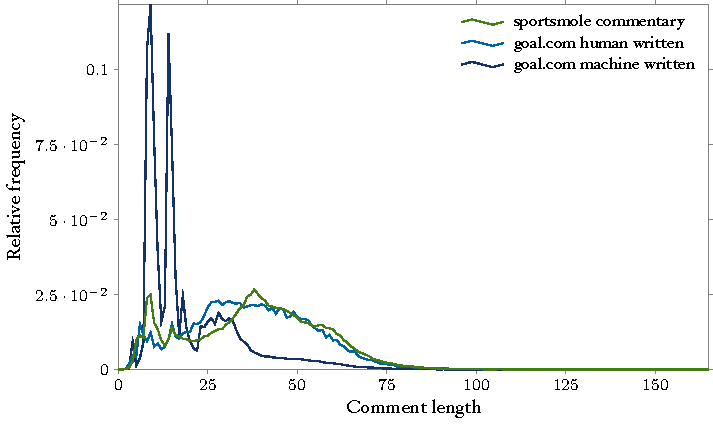
\includegraphics[width=\textwidth]{figures/fig_commentary_full.pdf}
\end{frame}

\begin{frame}
\frametitle{What's in a comment 2}
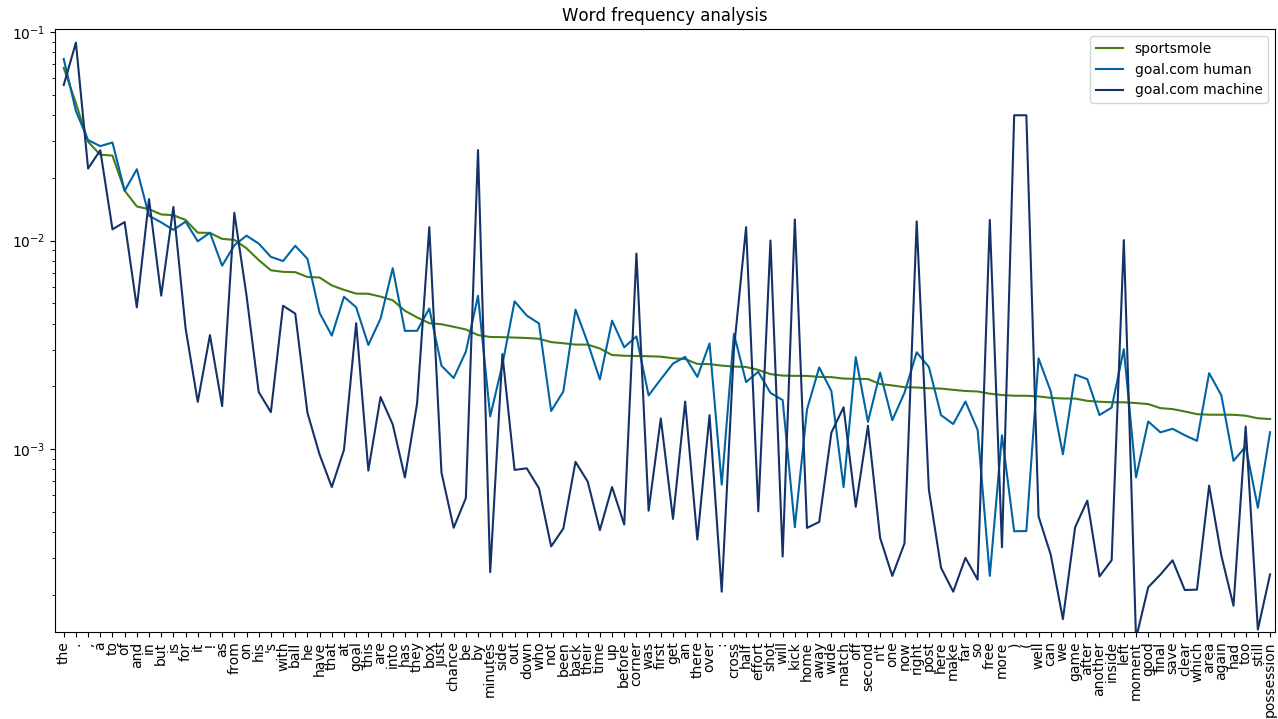
\includegraphics[width=\textwidth]{provider_comparison_hm}
\end{frame}

\begin{frame}
\frametitle{Power laws in language}
Words in a language are distributed according to a power law
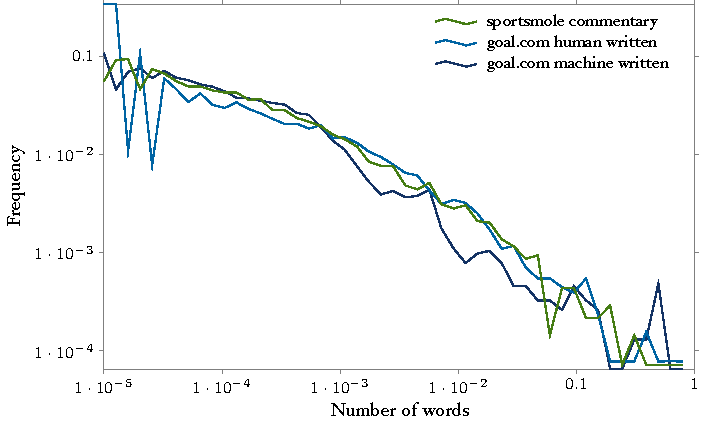
\includegraphics[width=.8\textwidth]{figures/fig_word_freq_full.pdf}
\end{frame}

\section{Word embedding}

\begin{frame}
\frametitle{Word representation}
\begin{itemize}
\item Words currently are just words, a bunch of strings without relation
\item If they are indexed ("the"=1, "a" = 2, "."=3), the words can be thought of as basis vectors in a $n$-dimensional space ($n$=\#words)
\item All words have the same distance to each other -> no relation
\item Is there a way to show word relations?
\end{itemize}
\end{frame}

\begin{frame}
\frametitle{word2vec/skip-gram}
Can embed the words into a lower-dimensional space (100 dims)\footnote{Mikolov et al: Distributed Representation of Words and Phrases and their Compositionality\\
Pennington et al: GloVe: Global Vectors for Word Representation}
Take a neural network and ask it to maximise the probability
\begin{align*}
\frac1n\sum_t \sum_c \log p(w_c, w_t)
\end{align*}
$n$ number of words, $t$ current word, $c$ context of the word, i.e. $\sum_c = \sum_{-c\le i \le c; j\ne 0} w_{t+i}$. Turn that into vectors,
\begin{align*}
p(w_i | w_t) = \frac{\exp\left({v_i}^\intercal v_t\right)}{\sum_j^n \exp \left({v_j}^\intercal v_t\right)} = \varphi(v_i^\intercal v_t)
\end{align*}
$v_t$ are the word vectors to be determined\\
Trivial solution: all $v_t$ the same
\end{frame}

\begin{frame}
\frametitle{Negative sampling}
Give the network some negative examples: maximise
\begin{equation*}
\max \left(\sum_{w,c \text{ valid}} \varphi_s \left(v_c^\intercal v_w\right) + \sum_{(w, c) \text{ not valid}} \varphi_s \left(-v_c^\intercal v_w\right)\right)
\end{equation*}
Negative examples can be randomly generated. Now what do we get from that?
\end{frame}

\begin{frame}
\frametitle{word to vectors}
\begin{itemize}
\item Word vectors $v_w$ now all live in the same space
\item Their relationship is based on the context of the word
\item Similar words will have similar context - Located close to each other in the embedding
\item Comparing vectors yields information about the text
\item Similarity queries and t-SNE
\end{itemize}
\end{frame}


\begin{frame}
\frametitle{Similarity queries 1}
\tiny
\begin{tabular}{r|c c c c c c c c}
Goal
 & $\begin{matrix}\text{defeat}\\0.419\end{matrix}$
 & $\begin{matrix}\text{leg}\\0.394\end{matrix}$
 & $\begin{matrix}\text{overhead}\\0.391\end{matrix}$
 & $\begin{matrix}\text{bicycle}\\0.379\end{matrix}$
 & $\begin{matrix}\text{victory}\\0.377\end{matrix}$
  & $\begin{matrix}\text{target}\\0.377\end{matrix}$
 & $\begin{matrix}\text{spot}\\0.358\end{matrix}$
 & $\begin{matrix}\text{post}\\0.354\end{matrix}$
\\\hline
Foul
 & $\begin{matrix}\text{lunge}\\0.756\end{matrix}$
 & $\begin{matrix}\text{trip}\\0.733\end{matrix}$
 & $\begin{matrix}\text{handball}\\0.728\end{matrix}$
 & $\begin{matrix}\text{tug}\\0.718\end{matrix}$
 & $\begin{matrix}\text{shove}\\0.705\end{matrix}$
 & $\begin{matrix}\text{challenge}\\0.676\end{matrix}$
 & $\begin{matrix}\text{tackle}\\0.656\end{matrix}$
 & $\begin{matrix}\text{simulation}\\0.619\end{matrix}$
\\\hline
Team
 & $\begin{matrix}\text{side}\\0.787\end{matrix}$
 & $\begin{matrix}\text{supporters}\\0.656\end{matrix}$
 & $\begin{matrix}\text{manager}\\0.629\end{matrix}$
 & $\begin{matrix}\text{outfit}\\0.605\end{matrix}$
 & $\begin{matrix}\text{record}\\0.558\end{matrix}$
 & $\begin{matrix}\text{club}\\0.546\end{matrix}$
 & $\begin{matrix}\text{fans}\\0.528\end{matrix}$
 & $\begin{matrix}\text{champions}\\0.524\end{matrix}$
\\\hline
Ronaldo
 & $\begin{matrix}\text{benzema}\\0.894\end{matrix}$
 & $\begin{matrix}\text{bale}\\0.872\end{matrix}$
 & $\begin{matrix}\text{griezmann}\\0.847\end{matrix}$
 & $\begin{matrix}\text{messi}\\0.823\end{matrix}$
 & $\begin{matrix}\text{neymar}\\0.786\end{matrix}$
 & $\begin{matrix}\text{isco}\\0.784\end{matrix}$
 & $\begin{matrix}\text{modric}\\0.783\end{matrix}$
 & $\begin{matrix}\text{morata}\\0.760\end{matrix}$
 \\\hline
Sweden
 & $\begin{matrix}\text{denmark}\\0.896\end{matrix}$
 & $\begin{matrix}\text{italy}\\0.885\end{matrix}$
 & $\begin{matrix}\text{porto}\\0.880\end{matrix}$
 & $\begin{matrix}\text{france}\\0.879\end{matrix}$
 & $\begin{matrix}\text{belgium}\\0.878\end{matrix}$
 & $\begin{matrix}\text{portugal}\\0.874\end{matrix}$
 & $\begin{matrix}\text{poland}\\0.871\end{matrix}$
 & $\begin{matrix}\text{russia}\\0.870\end{matrix}$
 \\\hline
Keeper
 & $\begin{matrix}\text{goalkeeper}\\0.808\end{matrix}$
 & $\begin{matrix}\text{mignolet}\\0.781\end{matrix}$
 & $\begin{matrix}\text{lloris}\\0.777\end{matrix}$
 & $\begin{matrix}\text{szczesny}\\0.768\end{matrix}$
 & $\begin{matrix}\text{begovic}\\0.764\end{matrix}$
 & $\begin{matrix}\text{speroni}\\0.754\end{matrix}$
 & $\begin{matrix}\text{guzan}\\0.754\end{matrix}$
 & $\begin{matrix}\text{schmeichel}\\0.752\end{matrix}$
 \\\hline
 $-$Goal
& $ \begin{matrix} \text{joins} \\ 0.381 \end{matrix}$
& $ \begin{matrix} \text{enters} \\ 0.373 \end{matrix}$
& $ \begin{matrix} \text{demands} \\ 0.367 \end{matrix}$
& $ \begin{matrix} \text{toward} \\ 0.362 \end{matrix}$
& $ \begin{matrix} \text{artificial} \\ 0.358 \end{matrix}$
& $ \begin{matrix} \text{flattens} \\ 0.355 \end{matrix}$
& $ \begin{matrix} \text{featuring} \\ 0.348 \end{matrix}$
& $ \begin{matrix} \text{cardnow} \\ 0.347 \end{matrix}$
\\\hline
$-$Foul
& $ \begin{matrix} \text{lacks} \\ 0.352 \end{matrix}$
& $ \begin{matrix} \text{around} \\ 0.345 \end{matrix}$
& $ \begin{matrix} \text{entire} \\ 0.337 \end{matrix}$
& $ \begin{matrix} \text{lacked} \\ 0.322 \end{matrix}$
& $ \begin{matrix} \text{onto} \\ 0.304 \end{matrix}$
& $ \begin{matrix} \text{complexion} \\ 0.300 \end{matrix}$
& $ \begin{matrix} \text{carousel} \\ 0.288 \end{matrix}$
& $ \begin{matrix} \text{cliché} \\ 0.286 \end{matrix}$
\\\hline
$-$Team
& $ \begin{matrix} \text{right-hand} \\ 0.474 \end{matrix}$
& $ \begin{matrix} \text{left-hand} \\ 0.460 \end{matrix}$
& $ \begin{matrix} \text{rescues} \\ 0.456 \end{matrix}$
& $ \begin{matrix} \text{well-positioned} \\ 0.432 \end{matrix}$
& $ \begin{matrix} \text{wrong} \\ 0.428 \end{matrix}$
& $ \begin{matrix} \text{outmuscles} \\ 0.413 \end{matrix}$
& $ \begin{matrix} \text{falls} \\ 0.405 \end{matrix}$
& $ \begin{matrix} \text{misdirected} \\ 0.399 \end{matrix}$
\\\hline
$-$Ronaldo
& $ \begin{matrix} \text{hounding} \\ 0.599 \end{matrix}$
& $ \begin{matrix} \text{outnumber} \\ 0.583 \end{matrix}$
& $ \begin{matrix} \text{pressurising} \\ 0.520 \end{matrix}$
& $ \begin{matrix} \text{bombarding} \\ 0.515 \end{matrix}$
& $ \begin{matrix} \text{playmaking} \\ 0.505 \end{matrix}$
& $ \begin{matrix} \text{harrying} \\ 0.503 \end{matrix}$
& $ \begin{matrix} \text{isbookedfor} \\ 0.493 \end{matrix}$
& $ \begin{matrix} \text{changeit} \\ 0.492 \end{matrix}$
\\\hline
$-$Sweden
& $ \begin{matrix} \text{loanee} \\ 0.495 \end{matrix}$
& $ \begin{matrix} \text{skipper} \\ 0.479 \end{matrix}$
& $ \begin{matrix} \text{over-play} \\ 0.474 \end{matrix}$
& $ \begin{matrix} \text{penalise} \\ 0.474 \end{matrix}$
& $ \begin{matrix} \text{substitutionfor} \\ 0.468 \end{matrix}$
& $ \begin{matrix} \text{foil} \\ 0.459 \end{matrix}$
& $ \begin{matrix} \text{hounding} \\ 0.445 \end{matrix}$
& $ \begin{matrix} \text{enner} \\ 0.441 \end{matrix}$
\\\hline
$-$Keeper
& $ \begin{matrix} \text{involving} \\ 0.536 \end{matrix}$
& $ \begin{matrix} \text{featuring} \\ 0.525 \end{matrix}$
& $ \begin{matrix} \text{fells} \\ 0.523 \end{matrix}$
& $ \begin{matrix} \text{xabi} \\ 0.452 \end{matrix}$
& $ \begin{matrix} \text{alongside} \\ 0.450 \end{matrix}$
& $ \begin{matrix} \text{talented} \\ 0.447 \end{matrix}$
& $ \begin{matrix} \text{aleix} \\ 0.443 \end{matrix}$
& $ \begin{matrix} \text{cesc} \\ 0.441 \end{matrix}$
 \end{tabular}
 \end{frame}

\begin{frame}
\frametitle{Similarity queries 2}
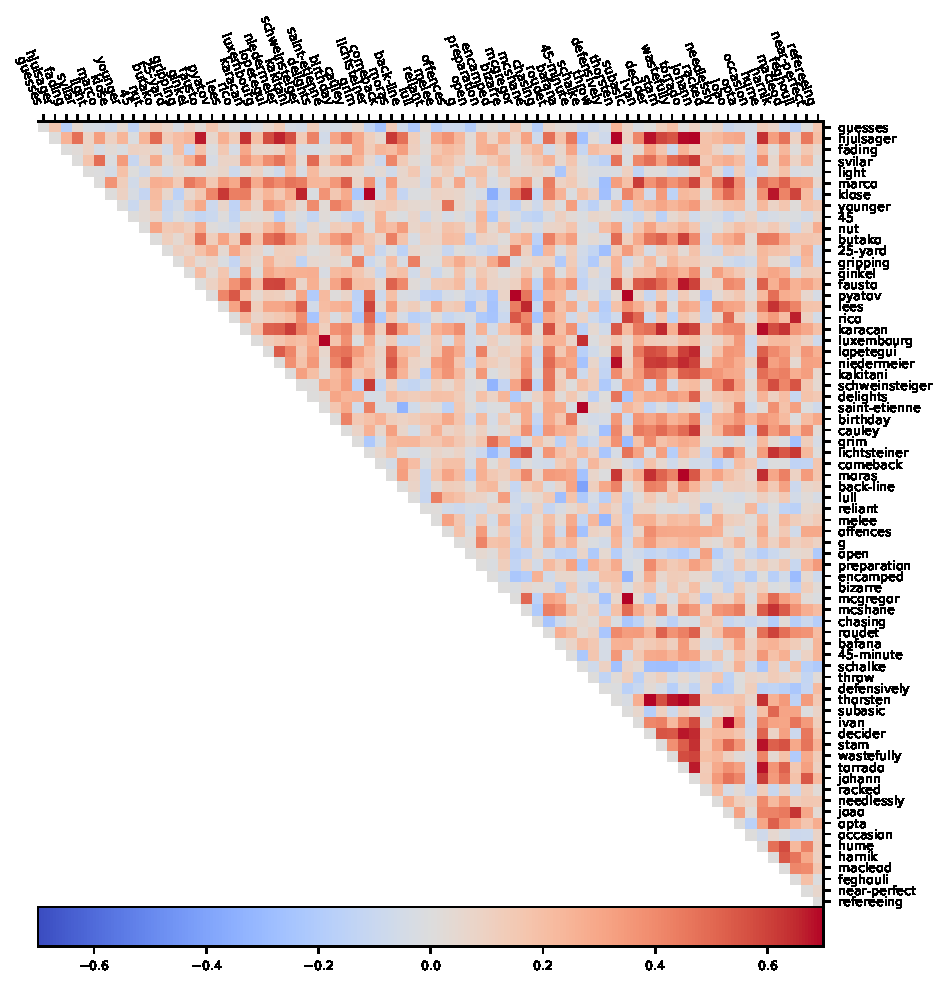
\includegraphics[width=.75\textwidth]{figures/similarity_matrix.pdf}
\end{frame}

\begin{frame}
\frametitle{Similarity queries 3}
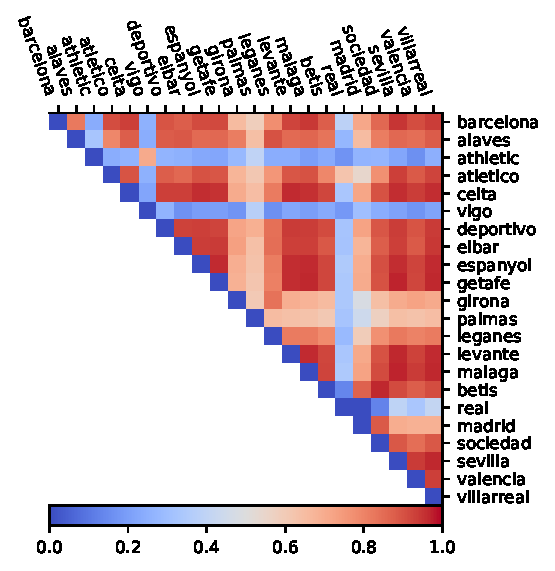
\includegraphics[width=0.49\textwidth]{figures/simmat_spanish_teams.pdf}
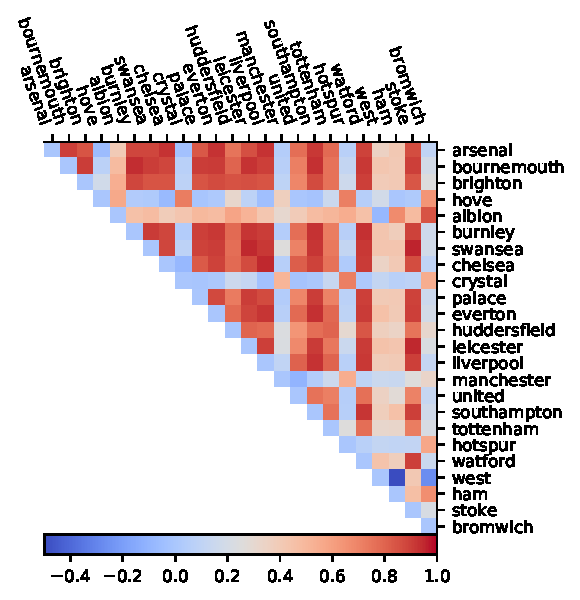
\includegraphics[width=0.49\textwidth]{figures/simmat_english_teams.pdf}
\end{frame}

\begin{frame}
\frametitle{t-SNE 1}
\begin{itemize}
\item The prior queries are word-to-word
\item What if one needs an overview of all words
\item Embed all words in 2D with t-SNE (t-distributed Stochastic Neighbourhood Embedding)\footnote{van der Maarten et al: Visualizing Data using t-SNE}
\item This returns a rough (not exact) picture of density variations and word relations
\end{itemize}
\end{frame}

\begin{frame}
\frametitle{t-SNE 2}
%\vspace{-2cm}
\includegraphics[width=0.5\textwidth]{figures/tsne_teams.pdf}
\includegraphics[width=0.49\textwidth]{figures/tsne_numbers.pdf}
\end{frame}



\section{Bias in writing}

\begin{frame}
\frametitle{The tale of the biased writer}
\begin{minipage}{0.75\textwidth}
\begin{itemize}
\item{With a whole text corpus at hand, one can ask the question: Are the authors biased?}
\item Take 9 adjectives and compare their number of appearances together with players
\item Are there significant outliers?
\item Is there a bias against a particular nationality?
\end{itemize}
\end{minipage}
\begin{minipage}{0.2 \textwidth}\small
\begin{tabular}{|l}
bad\\
poor\\
frustrated\\
amazing\\
great\\
fantastic\\
aggressive\\
angry\\
dangerous
\end{tabular}
\end{minipage}
\end{frame}

\begin{frame}
\frametitle{Players with too many adjectives 1}
\scriptsize
\begin{tabular}{r l r l}
Player (\#tags) & Attribute (\#found) & Expected & $p$-value\\\hline
Gayle (867) &great (13) & 4.9 & $0.9998$\\
Murray (982) &great (11) & 4.7 & $0.9982$\\
Ritchie (1102) &dangerous (11) & 5.0 & $0.9966$\\
{\color{gray}Naughton (631)} &{\color{gray}dangerous (12)} & {\color{gray}3.1} & {\color{gray}$0.9999$}\\
{\color{gray}Mcclean (606)} &{\color{gray}poor (11)} & {\color{gray}3.0} & {\color{gray}$0.9999$}\\
Lovren (1575) &dangerous (16) & 10.3 & $0.9614$\\
Smalling (1417) &dangerous (12) & 7.0 & $0.9717$\\
Brunt (1513) &dangerous (14) & 8.9 & $0.9646$\\
Barry (1491) &dangerous (11) & 6.7 & $0.9506$\\
Davis (1350) &poor (12) & 7.3 & $0.9592$\\
Davis (1350) &great (12) & 7.1 & $0.9691$\\
Reid (1260) &dangerous (11) & 5.7 & $0.9872$\\
Moreno (1238) &poor (12) & 6.7 & $0.9800$\\
Shaw (1264) &dangerous (11) & 5.7 & $0.9868$\\
Blind (920) &dangerous (13) & 4.9 & $0.9998$\\
Morrison (1186) &great (11) & 5.7 & $0.9873$\\
Cyne (1413) &great (14) & 8.6 & $0.9672$\\
Vorm (1070) &great (11) & 5.1 & $0.9953$\\\hline
\end{tabular}
\end{frame}

\begin{frame}
\frametitle{Players with too many adjectives 2}
\scriptsize%\hspace{-0.8cm}
\begin{tabular}{r l r l}
Nation (\#tags) & Attribute (\#found) & Expected & $p$-value\\\hline
Poland (2796) & great (14) & 8.6 & $0.9666$\\
 Germany (2925) & great (15) & 9.7 & $0.9571$\\
 Germany (2925) & dangerous (16) & 9.7 & $0.9782$\\
 Egypt (2918) & dangerous (14) & 8.5 & $0.9710$\\
 Ghana (2955) & dangerous (15) & 9.2 & $0.9721$\\
 Algeria (2808) & dangerous (25) & 14.6 & $0.9969$\\
 Algeria (2808) & great (12) & 7.4 & $0.9536$\\
 Iceland (2866) & dangerous (18) & 10.7 & $0.9873$\\
 Iceland (2866) & great (13) & 8.2 & $0.9529$\\
 Senegal (2682) & great (15) & 8.9 & $0.9804$\\
 Senegal (2682) & dangerous (12) & 6.7 & $0.9802$\\
 {\color{gray}United States (1187)} & {\color{gray}dangerous (11)} & {\color{gray}2.7} & {\color{gray}$1.0$}\\
 Norway (2071) & great (11) & 5.0 & $0.9962$\\
 Cameroon (1601) & poor (12) & 4.4 & $0.9999$\\
 Croatia (1715) & dangerous (17) & 6.1 & $0.9999$\\
 Croatia (1715) & poor (11) & 4.3 & $0.9993$\\
 DR Congo (3407) & dangerous (23) & 16.3 & $0.9527$\\
 New Zealand (1878) & dangerous (17) & 6.6 & $0.9999$\\
 New Zealand (1878) & poor (11) & 4.7 & $0.9980$\\
 New Zealand (1878) & great (11) & 4.6 & $0.9986$\\\hline
 \end{tabular}
 \end{frame}
 
 \begin{frame}
 \frametitle{Players with too few adjectives}
 \begin{itemize}
 \item Here there is a collection effect, common names are just grouped together and distort the statistic
 \item Only find first names that are common for one nation
 \item Same goes for grouping by nation
 \item Nothing to be learned here
 \end{itemize}
 \end{frame}
 
 \begin{frame}
 \frametitle{Adjectives by word2vec 1}
 \begin{itemize}
 \item Have seen that word vectors can represent similarities between words
 \item Can be used here: How similar is each player [name] to an adjective?
 \item Is there a significant difference to African players?
 \end{itemize}
 \end{frame}
 
 \begin{frame}
 \frametitle{Adjective by word2vec 2}
 \begin{tabular}{c c c}
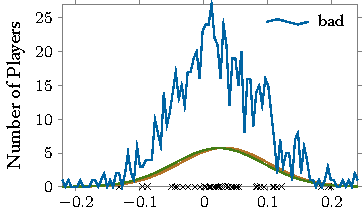
\includegraphics[width=0.3\textwidth]{figures/bad_distribution.pdf} & 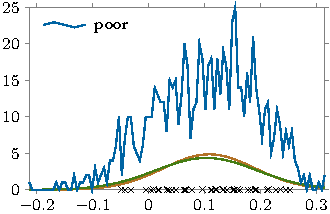
\includegraphics[width=0.3\textwidth]{figures/poor_distribution.pdf} & 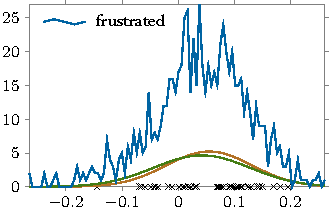
\includegraphics[width=0.3\textwidth]{figures/frustated_distribution.pdf}\\
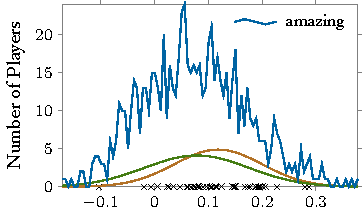
\includegraphics[width=0.3\textwidth]{figures/amazing_distribution.pdf} & 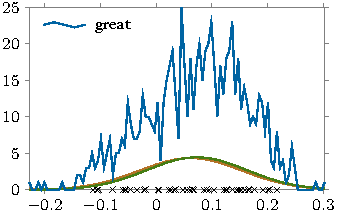
\includegraphics[width=0.3\textwidth]{figures/great_distribution.pdf} & 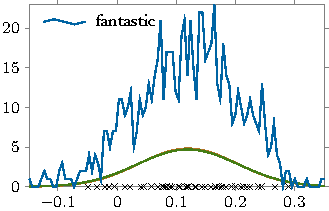
\includegraphics[width=0.3\textwidth]{figures/fantastic_distribution.pdf}\\
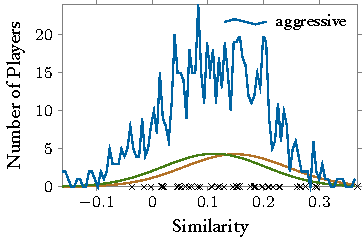
\includegraphics[width=0.3\textwidth]{figures/aggressive_distribution.pdf} & 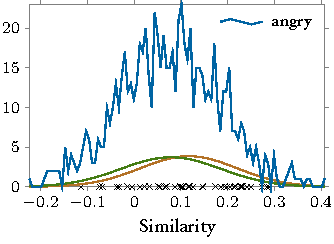
\includegraphics[width=0.3\textwidth]{figures/angry_distribution.pdf} & 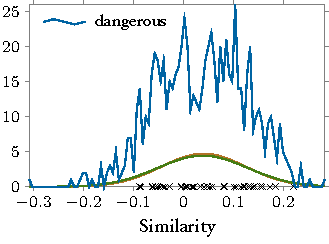
\includegraphics[width=0.3\textwidth]{figures/dangerous_distribution.pdf}
\end{tabular}
\end{frame}

\begin{frame}
\frametitle{Adjectives by word2vec 3}
\begin{itemize}
\item Most distributions look very similar, but what about the distributions that look different?
\item Use Kolmogorov-Smirnov test
\item Distributions for amazing and aggressive are different ($p<0.01$), angry might be ($p\approx0.05$)
\item The adjectives found here are not the same as the ones found before
\item No clear indication of a bias, but a number of starting points for a detailed analysis
\end{itemize}
\end{frame}

\section{Automatic comment generation}

\begin{frame}
\frametitle{Text creation 1}
\begin{itemize}
\item Now that the data is understood and examined, one can consider to extend it
\item For each word $w_t$, choose a context $w_{t-j} \in c_t$. Then for each $c_t$, there is a finite number of possible words $w_i$ that fit to it
\item Going through the whole text, note words $w_i$ to each context. Normalising gives a probability
\end{itemize}
\begin{align*}
p(w_t|c_t) = \begin{pmatrix} w_1 & p_1 \\\vdots & \vdots \\w_n & p_n\end{pmatrix}, \sum_{i=1}^n p_i = 1
\end{align*}
\begin{itemize}
\item This is maximum likelihood language modelling
\end{itemize}
\end{frame}

\begin{frame}
\frametitle{Text creation 2}
\begin{itemize}
\item Now do that automatically with a recurrent neural network
\item Word to word prediction:
\end{itemize}
\begin{align*}
p(w_t|w_{t-1}) = \left(\begin{array}{c c | c} w_1 &p_1& c_1\\\vdots & \vdots & \vdots \\ w_n & p_n & c_n\end{array}\right)
\end{align*}
\begin{itemize}
\item The context now includes all prior sentences
\item Can capture much longer dependencies
\item This is neural network language modelling
\end{itemize}
\end{frame}

\begin{frame}
\frametitle{Text creation 3}
\begin{itemize}
\item Test on a smaller model first
\item As an input, take the index of word (ordered by frequency)
\item As output, take the dimensions of highest value -> word
\item For faster training, take only a small word sample (Premier League 2017/18 in sportsmole
\item Do a couple of word replacements: \texttt{<player>}, \texttt{<team>}, \texttt{<unk>}, \texttt{<pad>}
\item This is the common approach
\end{itemize}
\end{frame}

\begin{frame}
\frametitle{Example output}
\begin{itemize}
\item Train the model, throw in a random word; What comes out?
\item The context here comes from training the model
\end{itemize}
\tiny
\begin{tabular}{l}
\hline
shots that been well off <team> his been more content to it , just an <unk> action when he <unk> he\\
goal four the second from goal . <pad> <pad> <pad> <pad> <pad> <pad> <pad> <pad> <pad> <pad> <pad> <pad> <pad> <pad>\\
a the former winger had taken yards out , but the effort was always <unk> away from goal . <pad> <pad>\\
this would about the hand of <unk> ? ! the <team> midfielder has just been booked for <unk> handball after sticking\\
this the former . <team> brom <unk> the <unk> has <unk> the bench that he is struggling . <pad> <pad> <pad>\\
his what about he <unk> he could n't reach it with his head . <pad> <pad> <pad> <pad> <pad> <pad> <pad>\\
<unk> had off reach <team> of the hand of <unk> , but what about the hand of <unk> ? ! the\\
shot lets the ball cross . there was not much intent to it , just an <unk> action when he <unk>\\
update winger . half-time change , taking off <player> . <pad> <pad> <pad> <pad> <pad> <pad> <pad> <pad> <pad> <pad> <pad>\\
this the bench . <team> brom <unk> the <unk> has <unk> the bench that he is struggling . <pad> <pad> <pad>\\
after off takes a <player> <unk> gets <unk> . <unk> that <player> to would have had a one-on-one had his line\\
alan off <player> <team> also gets into the box alongside the striker . <player> has only done that once so far\\\hline
\end{tabular}
\end{frame}

\begin{frame}
\frametitle{Analysis}
\begin{itemize}
\item This output approaches understandable
\item Has understood some parts of the language
\item Seems to work, promising indicator for the next step
\end{itemize}
\end{frame}

\begin{frame}
\frametitle{Large model}
\begin{itemize}
\item With a good start from the prior model, take on a larger one
\item Same word replacements (rebuild embedding)
\item Model appears to converge
\item But training time extremely slow, more than a week for one run over the whole text base
\item No meaningful output was created
\end{itemize}
\end{frame}

\section{Ball positions to text}

\begin{frame}
\frametitle{What to do}
\begin{itemize}
\item Can classify possession chains into different outcomes
\item Can create a comment based on initial word
\item Connect possession chains to a single word vector (as a proxy for the comment)
\end{itemize}
\end{frame}

\begin{frame}
\frametitle{Results}
\begin{itemize}
\item The connection between ball positions and all comments does not appear to work
\item Comments are much more than "goal", "throw-in"…
\item A lot of the commentary describes the general match situation rather than relating directly to actions in the field
\end{itemize}
\end{frame}

\begin{frame}
\frametitle{Conclusions \& Outlook}
\begin{itemize}
\item Neural networks manage to emulate analytical conditions and classify structures
\item A simpler model may well be successful, based on a limited number of conditions which in turn are linked to appropriate comments
\item The question of whether a bias exists in the text base merits  examination
\end{itemize}
\end{frame}
%\begin{frame}
%\frametitle{Text creation 4}




\end{document}
